%! Author = louis
%! Date = 28-10-22

% Preamble
\documentclass[12pt, a4paper, oneside]{article}

% Packages
\usepackage[french]{babel}
\usepackage[margin=2.5cm]{geometry}
\usepackage[utf8]{inputenc}
\usepackage{graphicx}
\usepackage[colorlinks=true, pdfborder {0 0 0},linkcolor=black]{hyperref}
\usepackage{listings}
\usepackage{color}
\usepackage{lipsum}
\usepackage[nomain, toc, xindy, acronym]{glossaries}
\usepackage{wrapfig}
\usepackage{fancyhdr}
\usepackage[T1]{fontenc}
\usepackage[labelformat=empty]{caption}
\usepackage{titlepic}
\usepackage[xindy]{imakeidx}
\usepackage[backend=bibtex]{biblatex}
\usepackage{pdfpages}
%\usepackage{plantuml}
\usepackage{float}
\hypersetup{
    colorlinks=true,
    linkcolor=black,
    filecolor=magenta,
    urlcolor=cyan,
    pdftitle={Clever-Party-Thrower, une application web hébergée via Kubernetes et Ansible},
    pdfpagemode=FullScreen,
}
\fancyhf{}
\fancyhead[LO,RE]{\sffamily\itshape \leftmark}
\fancyfoot[C]{\thepage}
\pagestyle{fancy}

\makeatletter
\renewcommand\paragraph{\@startsection{paragraph}{4}{\z@}%
% display heading, like subsubsection
{-3.25ex\@plus -1ex \@minus -.2ex}%
{1.5ex \@plus .2ex}%
{\normalfont\normalsize\bfseries}}
\setcounter{secnumdepth}{4}
\makeatother
% Document
\begin{document}
    \begin{titlepage}
        \begin{center}
            \vspace*{1cm}

            \Huge
            \textbf{Clever-Party-Thrower, une application web hébergée via Kubernetes et Ansible}

            \vspace{0.5cm}

            \vspace{1.5cm}

            \textbf{Louis De Wilde}

            \vfill

            \includegraphics[width=0.65\textwidth]{images/EPHEC_logo.svg}
            \vfill
            \vspace{0.8cm}
            \Large
            Technologie de l'informatique 3TL2 \\
            Ephec : Av. du Ciseau 15, 1348 Ottignies-Louvain-la-Neuve\\
            Novembre 2022

        \end{center}
    \end{titlepage}
    \thispagestyle{empty}
    \newpage
    \setcounter{page}{0}
    \begin{KeepFromToc}
        \tableofcontents
    \end{KeepFromToc}
    \newpage
    % \bibliography{main}
    %\bibliographystyle{plain}


    \section{Introduction}\label{sec:introduction}
    

Dans le monde d'aujourd'hui, les étudiants et les personnes en général sont souvent amenés à organiser des événements, tels que des soirées ou des fêtes entre amis.
Cependant, gérer les aspects logistiques de ces événements peut s'avérer compliqué, notamment lorsqu'il s'agit de fixer une date, de répartir les coûts et de coordonner les participants.
Afin de faciliter ce processus et d'améliorer l'expérience de l'organisation de fêtes, j'ai décidé de développer une application web nommée "Clever Party Thrower".
Cette application permettra aux utilisateurs de gérer efficacement tous les aspects importants de l'organisation d'un événement,
y compris les dépenses, les courses voir meme les covoiturages, la musique et bien plus encore.\\\\

Dans ce rapport, je présenterai les différentes étapes du développement de l'application Clever Party Thrower,
en commençant par le choix du sujet et en détaillant le cahier des charges, l'analyse de la problématique, la conception et la réalisation du projet.
J'aborderai également les aspects liés à la sécurité, la gestion des versions, les tests et la documentation du code.\\
Un accent particulier sera mis sur l'adoption de pratiques de développement modernes, telles que l'intégration continue (CI) et le déploiement continu (CD), afin d'assurer la qualité et la fiabilité du code tout au long du cycle de développement.
De plus, je discuterai des choix d'hébergement pour l'application, en explorant les options d'auto-hébergement voir meme compatible avec le cloud.\\

Enfin, je terminerai en présentant une conclusion sur le travail accompli, les défis rencontrés et les perspectives d'amélioration pour le futur.
    \newpage


    \section{Choix du sujet}\label{subsec:choix-du-sujet}
    
Dans le contexte actuel, les étudiants et les personnes qui aiment s'amuser en général organisent souvent des soirées ou des fêtes entre amis.
Pourtant, planifier et organiser de tels événements peut s'avérer difficile, en particulier lorsqu'il s'agit de fixer une date convenant à la majorité des participants et de gérer les dépenses.
Les défis augmentent lorsque le nombre de participants s'accroît.

Afin de résoudre ce problème, j'ai décidé de créer une application web qui facilite l'organisation de petites fêtes estudiantines.
Ce sujet présente un intérêt technique, car il implique la création d'une plateforme en ligne accessible à un large public.
De plus, il répond à un besoin réel des utilisateurs qui cherchent à simplifier l'organisation de leurs événements et à réduire les efforts nécessaires pour coordonner les participants.

L'application apportera une plus-value en proposant des fonctionnalités spécifiques pour gérer les aspects clés de l'organisation d'une fête, telles que la répartition des coûts,
la gestion des courses et le choix d'une date.
En outre, elle offrira un positionnement unique par rapport aux solutions existantes en offrant toutes ces fonctionnalités au sein d'une meme application.

Enfin, le sujet a été validé par un cours sondage au pres d'une vingtaine d'étudiants et une recherche d'application similaire deja existante, qui ont montré un intérêt pour une telle solution.
Ce travail représentera une charge de travail suffisante, estimée à environ 350 heures.
    \newpage


    \section{Cahier des charges}\label{sec:cahier-des-charges}
    %! Author = louis
%! Date = 28-10-22

\subsection{Choix du sujet}\label{subsec:choix-du-sujet}
En tant qu’étudiant (ou personnes aimant nous amuser de manière générale), nous sommes souvent amenés à organiser une soirée ou une fête entre amis.
Il faut alors trouver une date qui convient au au plus grand nombre et gérer les dépenses de la fête, ce qui peut s'avérer compliqué quand le nombre de participants augmente.
C’est pourquoi j’ai décidé de créer une application web facilitant l’organisation de petites fêtes estudiantines.

\subsection{Cahier des charges}\label{subsec:cahier-des-charges}

\subsubsection{Besoin du client}
\begin{itemize}
    \item Permet de répartir équitablement les frais engendrés par la fête
    \item Permet de créer une playlist commune (sur laquelle chacun a la possibilité d'ajouter des titres)
    \item Crée une liste des courses pour la soirée (éventuellement une répartition si toutes les courses ne se font pas au meme endroit ?)
    \item Connaître qui a amène quoi à la fête
    \item Crée différents évènements
    \item Est accessible grâce à un simple lien
    \item Est pourvu d'un système de connexion et de création de compte simple
    \item Permet de trouver une date d’évènement qui convient au plus grand nombre de participants
    \item Permet au participant d'organiser facilement des covoiturages
    \item Permet au conducteur de connaitre son trajet de covoiturage
    \item Calcule et reparti automatiquement les frais de transport entre les différents covoitureurs
\end{itemize}

\subsubsection{Contraintes}
\begin{itemize}
    \item Accessible sur toutes les plateformes (Android, IOS, Mac, Windows, Linux)
    \item Le système de création de compte doit être simple
    \item Les données des utilisateurs seront sécurisées
    \item L’application doit être auto-hébergable
\end{itemize}

\subsubsection{Méthodologie}
N’ayant pas de client autre que moi, je ne compte pas appliquer de méthodologie vraiment spécifique (comme scrum par exemple).\\
En revanche, je vais m’inspirer de cette dernière en divisant les demandes de l’utilisateur en petites tâches.\\
Afin de suivre l’avancement du projet et de m’organiser au mieux, j’utiliserai FocalBoard, qui me servira à créer des cartes représentant les différentes tâches et me permettra de les gérer visuellement.\\
Le code, quant à lui, sera géré sur \href{https://github.com/craftbrak/Clever-Party-Thrower}{Github}\footnote{\url{https://github.com/craftbrak/Clever-Party-Thrower}}.
Je voudrais si possible, pour certaines parties du projet, utiliser de l'intégration voire du déploiement continu, en plus de tests automatisés.
    \newpage


    \section{Analyse}\label{sec:analyse}
    %! Author = louis
%! Date = 28-10-22

Le projet ayant comme contrainte pricipale d'etre disponible sur toute les platformes majeur une base web me parait évident.
pourtant le web viens aussi avec la limitation pricipale qu'est le besoin de connection permanente au serveur,
pour remedier a ce probleme un PWA (Application Web Progressive) nous permetrais de beneficiez des avantages du web,
tout en permetant aux utilisateurs de concerver une version locale de l'application.
De plus une PWA permet d'etre instalée comme une application native Android ou IOS pour les platformes mobiles ce qui facilite l'accès.\\\\

Une PWA comme toute application web necesite plusieurs composant:
\begin{itemize}
    \item Un back-end
    \item une Base de Donnée
    \item une Interface definie pour le back-end (API)
    \item un front-end
\end{itemize}
\subsection{Back-end}\label{subsec:back-end}
Le serveur back-end doit etre capable de mettre a disposition les donnée nescesaire au fonctionnement de l'application.
Cependant le back-end sera aussi responcable des calcul d'equilibrage des depence , des matching de covoiturage et des trajets.
Connaissant deja Express.js et Spring (Kotlin) je me suis naturellement tourner vers ce derniers néanmoins je desirais utiliser du TypeScript pour ce projet.
Express.js est compatible avec TypeScript mais Spring ne l'est pas, Express.js est leger, minimaliste et propose une bonne documentation,
Spring est generaliste propose des outils de generation de code et utilise une systeme d'injection de dependance.
Ce qu'il me falais etait une hybride entre Spring et Express.js.
Apres quelque recherche j'ai trouver un framework appler Nest.js, ce dernier supporte nativement TypeScript, propose une documentation ecxelante,
propose un CLI permetant de generer du code boiler plate, reste simple et leger, Utilise de l'injection de dependance et est tres utiliser et apprecier par d'autre developeurs.
J'ai donc decider d'utiliser Nest.Js pour ce projet.

\subsubsection{ORM}
Nest.Js (que je vais appeller Nest a partir de maintenant) n'est pas un framework batteries included comme le son Spring ou Larravel,
Il m'a donc fallu choisir aussi un ORM pour interfacer avec ma base de donnée.
Dans la Documentation de Nest, il y a des exemple de configuration avec les ORM les plus Utiliser avec Nest et TypeScrip.
Ces derniers sont Sequelize, TypeOrm et Prisma ,
ayant eu une experience avec Sequelize plus tot mauvaise lors de mon projet de dev3, j'ai decider de regarder du coté de prisma.
Prisma est une ORM un peu particulier dans le sens ou il propose d'utiliser une schema prisma pour definir ces entité plutot que le code TypeScript.
Cella me parraissait une tres bonne chose vu que prisma generais alors lui meme les differents DTO nescesaire.
Il c'est cependant averer que a l'utilisation prisma n'est pas l'ideale surtout lorsque l'on desire le coupler a une API graphQl
A cause de son schema particulier je devais definir le forma de mes entitée a 2 endroit et tout de meme crée manuelement mes DTO
J'ai donc decider de jeter une oeuil a TypeOrm, celui ci propose de definir les entité via des anotation TypeScript.
Ce qui me permet d'utiliser une seule classe pour definir mon entitée d'orm et de graphQl de plus TypeOrm est mieux
documenter grace au support d'une comunauter plus large.


\subsection{La base de donnée}\label{subsec:la-base-de-donnee}
Ma base de donnée devais me permetre 2 chose, stocker des donnée geographique et faire des operation sur ces donnée.
Le seul choix qui s'offrais a moi compatible avec TypeOrm etait postgress avec une extention nomer POSTGIS.
Postgres est une base de donnée tres utiliser en production et est tres performante et stable.

\subsection{L'API back end}\label{subsec:l'api-back-end}
Il existe plusieurs type d'API tres utiliser pour le Back-end mais les plus populaire sont le REST et le SOAP.
SOAP est de moin en moin utiliser du a la complexité intrinsec du xml et a ca lourdeur.
Il nous reste donc REST qui est une bonne solution mais nescecite pour presque chaque requete de recuperer des donnée qui ne seront pas toujour consomée par le client
Avec Rest l'on recupere une entitée complete tout les champs sont renvoyer.
C'est pour cela que graphQl a ete crée , non seulement graphQL utilise un typage fort via un schema defini et exposer par le serveur,
mais en plus graphql permet de ne recuperer que les champs nescesaire au client grace au GQL.




\subsection{Front-end}\label{subsec:front-end}
Pour ce qui est de l'interface utilisateur ( le front end ) j'ai decidé d'utiliser angular car ce framework utilise TypeScript nativement et supporte aussi les PWA
TypeScript est important car il permet de eliminer les bugs lier au typage d'objet avant meme l'execution du programe.
Angular etant un framework orienter m'oblige aussi à suivre une architecture propre qui permet de rendre independant les differents composants du projet.


    \newpage


    \section{Hebergement et aspects reseaux}\label{sec:hebergement-et-aspects-reseaux}
    Afin d'héberger Clever Party Thrower, plusieurs possibilités s'offrent au client.
Celles-ci dépendent de son budget, de l'infrastructure dont il dispose et du nombre d'utilisateurs qui devront être servis.

\subsection{docker-compose}\label{subsec:docker-compose}
L'application, étant packagée dans des conteneurs Docker, peut être déployée très facilement dans un environnement restreint grâce à Docker et Docker Compose.
Durant le développement de l'application, j'ai souhaité permettre à des utilisateurs potentiels du service de tester certaines parties de l'interface.\\

J'ai donc décidé d'héberger un stack Docker Compose sur un petit serveur de mon homelab.
Le stack que j'ai choisi de décrire dans la documentation est minimaliste, il comprend le strict nécessaire pour héberger et utiliser l'application.
Le fichier docker-compose comprend le backend, la base de données et le frontend hébergé par un serveur nginx.

\subsection{kubernetes}\label{subsec:kubernetes}
Lorsque le client dispose d'une infrastructure performante, il a la possibilité de déployer l'application sur un ou plusieurs clusters Kubernetes.
Durant le développement de l'application, je me suis intéressé à l'orchestration de conteneurs avec Kubernetes,
ce qui m'a conduit à proposer des fichiers de configuration pour héberger le site web et son serveur.\\

En parallèle de ma formation sur Kubernetes, j'ai également exploré Ansible et ai adapté un projet open-source existant afin de permettre le déploiement de Clever Party Thrower sur un cluster Kubernetes en une seule commande.
Ce playbook Ansible facilite le déploiement d'un cluster K3S complet, avec ou sans haute disponibilité.
De plus, le playbook déploie également des applications telles que kubeVip, MetalLB, Rancher, Traefik, Cert-manager, LongHorn et ArgoCD.

\subsubsection{Le Playbook}
Le Playbook permet de déployer Kubernetes sur plusieurs machines, appelées nodes, afin d'ajouter de la résilience au cluster.
Plus il y a de nodes, plus le cluster peut en perdre sans interruption de service.
Les différentes applications utilisées pour permettre cette haute disponibilité sont les suivantes : \\

\begin{itemize}
    \item \textbf{Kubernetes} : Kubernetes synchronise et répartit toutes les configurations et les ressources entre les différentes nodes
    pour garantir que chacune d'entre elles peut à tout moment gérer le trafic.\\

    \item \textbf{Kubevip} : Kubevip sert à créer une adresse virtuelle pour la gestion du cluster.
    Cette adresse virtuelle permet de conserver une connexion avec le cluster tant qu'au moins une des nodes master est en ligne et fonctionnelle .\\

    \item \textbf{MetalLB} : MetalLB est un load balancer qui, comme son nom l'indique, permet d'équilibrer la charge de travail.
    Il attribue également des adresses IP à des pods (conteneurs dans Kubernetes) en fonction de leur nom ou espace de nom et ce, dans une plage définie .\\

    \item \textbf{Cert-manager} : Cert-manager permet de créer et renouveler les différents certificats via Let's Encrypt,
    en plus de permettre à Kubernetes de les gérer comme toute autre ressource, et donc de les synchroniser entre les différentes nodes.\\


    \item \textbf{Traefik} : Traefik sert de reverse proxy, protégeant ainsi les différents services du cluster.
    Il gère également la distribution de la charge pour les requêtes HTTPS .\\
    \item \textbf{Longhorn} : Longhorn permet de créer des volumes partagés et disponibles sur plusieurs nodes en même temps,
    garantissant ainsi aux pods exploitant ces volumes qu'ils seront toujours accessibles.\\
\end{itemize}

\subsection{Les Conteneurs}\label{subsec:les-conteneurs}
Le conteneur back-end est relativement simple.
Il utilise une image node:latest.
Une fois le code source transpilé, le résultat de cette compilation est copié dans l'image.\\

Le conteneur pour la base de données utilise quant à lui une simple image de PostGIS.
PostGIS est une extension de PostgreSQL qui permet la manipulation de points géographiques directement sur la base de données.\\

Le conteneur front-end est plus complexe.
Basé sur une image nginx, il intègre le résultat de la compilation Angular dans le dossier où nginx cherche les fichiers à servir.
Nginx sert donc le front end, et agit également comme un proxy pour permettre au front end d'accéder au backend.

\subsection{Mon choix}\label{subsec:mon-choix}
En tant que client, j'ai choisi d'héberger l'application via docker-compose.\\

À l'origine, mon objectif était de créer un cluster Kubernetes distribué entre plusieurs machines virtuelles pour simuler
diverses machines physiques, et de déployer l'application sur ce cluster.
Cependant, Kubernetes, et surtout la haute disponibilité, exige beaucoup de ressources, que mon serveur ne pouvait pas supporter.
Les différentes machines virtuelles manquaient constamment de mémoire ou d'espace disque.\\

J'ai ainsi décidé d'utiliser un simple docker-compose pour optimiser les ressources de mon serveur,
permettant d'héberger toutes mes applications plutôt que de se limiter à une seule avec des performances médiocres.
À l'avenir, si les limites matérielles ne sont plus un obstacle, j'envisagerai de déployer une infrastructure Kubernetes via Ansible,
avec l'ajout d'un système de surveillance.

\subsection{Sécurité et hébergement}\label{subsec:securite-et-hebergement}
Étant donné que le client est potentiellement responsable de l'hébergement de l'application, une grande partie des
responsabilités en termes de sécurité lui revient.
L'application doit être hébergée derrière un reverse proxy pour assurer la terminaison SSL, par exemple.
Les deux différentes méthodes d'hébergement assurent la sécurité de la base de données via le réseau Docker : seul le backend
a accès à la base de données.\\

Les différentes applications sont maintenues à jour soit via ArgoCD sur Kubernetes, soit via Watchtower sur Docker Compose.
Ces deux applications surveillent l'état du dépôt Docker Hub en temps réel et mettent à jour les services lors d'un changement.\\

Pour mon installation, j'ai choisi de faire confiance à Cloudflare pour sécuriser mon hébergement.
J'utilise un tunnel et leur reverse proxy afin de garantir la sécurité de mes services.
Cloudflare gère non seulement les certificats, mais permet aussi de bloquer les attaques de type DDoS. De plus, grâce au tunnel,
je n'ai pas à configurer mon pare-feu sur mon router ni à exposer mon adresse IP publique.\\

À l'avenir, j'aimerais utiliser un pare-feu comme PfSense/OpenSense pour me permettre de faire du port forwarding directement
tout en garantissant la sécurité de l'application.\\

De plus, lorsque l'application sera hébergée sur un cluster Kubernetes, la gestion des certificats et de la terminaison
SSL sera effectuée par le cluster et non par un tier de confiance comme cloudflare.\\

La configuration actuelle obtenue via le playbook Ansible met déjà en place un certificat privé pour l'application, géré par Certmanager,
ce qui le rend hautement disponible.
Cette disponibilité me permettra d'utiliser plusieurs instances concurrentes de Traefik réparties entre les différentes nodes du cluster.

\subsection{Performance et résilience à la charge}\label{subsec:performance-et-resilience}

Pour assurer la performance et la résilience à la charge de l'application Clever Party Thrower, plusieurs stratégies ont été mises en place .\\

\begin{itemize}
    \item \textbf{Réplication de conteneurs} : Grâce à Kubernetes, il est possible de déployer plusieurs instances de l'application sur différentes nodes.
    Cette approche permet d'améliorer la disponibilité de l'application en cas de panne sur une node, et également de répartir la charge utilisateur entre plusieurs instances.\\

    \item \textbf{Load balancing} : Utiliser un load balancer comme MetalLB dans un environnement Kubernetes permet de distribuer efficacement le trafic réseau entre plusieurs pods.
    Cela améliore la répartition de la charge et réduit le risque de surcharge d'une seule instance, ce qui se traduit par une meilleure performance globale de l'application .\\

    \item \textbf{Scalabilité horizontale} : La scalabilité horizontale, qui consiste à ajouter plus de nodes à un cluster, est une autre stratégie pour gérer une charge croissante .
    Avec l'aide de Kubernetes et de son fonctionnement basé sur des clusters, cette scalabilité peut être réalisée de manière relativement simple .\\

    \item \textbf{Gestion des ressources} : Kubernetes offre également des outils pour contrôler la quantité de ressources CPU et de mémoire que chaque pod peut utiliser .
    Cela permet de prévenir les situations où un pod consomme trop de ressources et affecte la performance des autres pods .\\

    \item \textbf{Volumes partagés avec Longhorn} : Longhorn assure la haute disponibilité des données en permettant de créer des volumes partagés et accessibles sur plusieurs nodes simultanément .
    Cela garantit que les pods exploitant ces volumes peuvent toujours y accéder, même en cas de défaillance d'une node .\\
\end{itemize}

Ainsi, en utilisant les outils et les principes de conception appropriés, il est possible de créer une application qui peut gérer efficacement une charge élevée tout en conservant une performance satisfaisante.
Dans le futur, des outils de surveillance et d'alerte pourraient être ajoutés pour assurer une détection proactive des problèmes de performance et permettre une intervention rapide en cas de problèmes.

\subsection{Schemas Réseau}\label{subsec:schemas-reseau}

\begin{figure}[H]
    \centering
    \begin{subfigure}[b]{0.45\textwidth}
        \includegraphics[width=\textwidth]{./images/shemaReseauDocker.drawio}
        \caption{Schema reseau Logique avec Docker}
        \label{fig:schemaDocker}
    \end{subfigure}
    \hfill
    \begin{subfigure}[b]{0.45\textwidth}
        \includegraphics[width=\textwidth]{./images/shemaReseauKube.drawio}
        \caption{Schema reseau Logique avec Kubernetes}
        \label{fig:schemaKube}
    \end{subfigure}
    \caption{Le sens des differents fleches represente le sens d'initialisation des connection}
    \label{fig:schemaReseau}
\end{figure} %todo: parler du reseau derier l'infra ce qui devrai etre fait
    \newpage


    \section{Développement de l'application}\label{sec:developpement-de-l'application}
    \subsection{Introduction}\label{subsec:introduction}
Cette section introduit l'architecture, la documentation du code, les bonnes pratiques de programmation, les tests unitaires et la sécurité de l'application web Clever Party Thrower.

\subsection{Architecture}\label{subsec:architecture}
Clever Party Thrower est une application web full-stack.
Le front-end est construit avec Angular tandis que le back-end est un monolithe élaboré avec NestJS et TypeORM. À chaque accès au site par un utilisateur,
la Single Page Application (SPA) Angular est chargée, initiant les services nécessaires pour interagir avec le back-end.
Ces services récupèrent les données requises via l'API GraphQL, en utilisant Apollo.\\

Durant toute la session de l'utilisateur, ces services persistent et continuent de récupérer les données du back-end au fur et à mesure de la navigation.
Chaque service est responsable d'un type de données spécifique.
Par exemple, AuthService s'occupe des données liées à l'authentification et à l'utilisateur, tandis qu'EventService gère tout ce qui est directement lié à un événement.\\

De la même manière, le back-end est divisé en plusieurs services, chacun gérant une ressource unique.
Ces services sont rassemblés en modules, associés aux contrôleurs REST et aux résolveurs GraphQL. Cette modularité facilite le test du code en assurant un découplage
entre les différents services.\\

\subsection{Documentation du code}\label{subsec:documentation-du-code}
Le code de Clever Party Thrower est organisé et documenté pour faciliter sa compréhension et sa maintenance.\\
Grâce à TypeScript, la majorité de la documentation est implicite.
Les noms des fonctions et leurs arguments offrent une compréhension rapide de leur utilité.
Pour les fonctions plus complexes, des commentaires expliquent la logique algorithmique.\\
Ainsi, même un développeur novice dans le projet peut facilement naviguer dans le code.

\subsection{Bonnes pratiques de programmation}\label{subsec:bonnes-pratiques-de-programmation}
Clever Party Thrower suit les conventions de codage d'Angular et de NestJS, ce qui comprend l'utilisation appropriée des indentations,
des commentaires, de la casse des lettres (camelCase, PascalCase), et des conventions de nommage des variables, des fonctions et des classes.
Cette pratique améliore la lisibilité du code et facilite le travail en équipe.\\

De plus, le code est divisé en modules et services distincts, chacun étant responsable d'une fonctionnalité spécifique.
Cela favorise la modularité, permet une meilleure gestion du code et facilite la maintenance et l'extension de l'application.\\

Les principes DRY (Don't Repeat Yourself) et SOLID sont également respectés pour minimiser la duplication de code et assurer la prédictabilité du comportement du logiciel.
Quelques concepts de programmation fonctionnelle sont utilisés dans le front-end, tels que l'immutabilité et l'utilisation maximale de fonctions pures.\\

La gestion des erreurs en JavaScript et TypeScript est plus basique que dans d'autres langages de programmation.
Contrairement à Java, où les erreurs doivent être déclarées dans la définition de la fonction, TypeScript ne possède pas cette fonctionnalité.
Il est donc difficile de savoir quelle fonction peut lancer une erreur.
La meilleure pratique est d'utiliser des blocs try-catch au niveau le plus élevé de l'application pour capturer les erreurs une fois qu'elles sont propagées.\\

\subsection{Tests Unitaires}\label{subsec:tests-unitaires}
Les tests unitaires sont une partie essentielle de Clever Party Thrower.
Chaque module et service dispose de ses propres tests unitaires, garantissant ainsi que chaque partie de l'application fonctionne comme prévu.
Les tests sont écrits avec Jest, un framework de test populaire pour JavaScript et TypeScript.\\

Le découplage des services et des modules rend les tests plus simples et plus efficaces, car chaque test se concentre sur une seule unité de code.

\subsection{Sécurité}\label{subsec:securite}
La sécurité est une préoccupation majeure pour Clever Party Thrower.
Parmi les mesures de sécurité mises en place, on compte l'utilisation de HTTPS pour toutes les communications via un reverse proxy dans l'infrastructure d'hébergement,
l'authentification et l'autorisation basées sur des tokens JWT, la validation des entrées côté serveur pour prévenir les attaques par injection,
et le chiffrement des données sensibles comme les mots de passe avant leur enregistrement en base de données avec argon2.
Les vulnérabilités potentielles sont régulièrement évaluées et des mises à jour de sécurité sont appliquées dès que nécessaire via npm audit et npm audit fix.

\subsubsection{RGPD}
Un aspect important de la sécurité de l'application est la protection des données.
L'application ne collecte pas de données autres que celles introduites via les différents formulaires.
La suppression des données est un sujet qui m'a demandé pas mal de réflexion.
Je ne pouvais pas simplement supprimer toutes les données liées à un utilisateur, car cela affecterait les autres utilisateurs qui partagent des événements ou des dépenses avec l'utilisateur à supprimer.
Plusieurs solutions s'offraient donc à moi : tout supprimer, mais dégrader grandement l'expérience pour les autres utilisateurs, remplacer l'utilisateur par un utilisateur anonyme par défaut, ou anonymiser l'utilisateur en changeant les données personnelles.
La solution de remplacer l'utilisateur complet risque tout de même de dégrader l'expérience des utilisateurs notamment au niveau du système de dettes.
J'ai alors opté pour la troisième solution et j'ai décidé de changer uniquement les données personnelles de l'utilisateur afin de l'anonymiser sans pour autant impacter les autres utilisateurs.

\subsection{GraphQL}\label{subsec:graphql}
L'utilisation de GraphQL pour l'API du projet a été une décision qui a parfois compliqué le développement de l'application.
Plusieurs difficultés ont été rencontrées, en particulier lors de la mise en place de la base de données avec Prisma.\\

Prisma et GraphQL fonctionnent tous deux sur la base d'un schéma, ce qui semble idéal en théorie.
Cependant, ces deux schémas sont construits via des outils différents, ce qui implique une maintenance manuelle de deux schémas séparés, susceptible d'introduire des erreurs.
Alternativement, il est possible d'utiliser des outils pour générer le schéma GraphQL ou Prisma à partir de l'autre, mais cette approche a aussi ses inconvénients.\\

Dans ma première approche, j'ai décidé de créer un schéma Prisma et de générer sur cette base le schéma GraphQL. Cette méthode, impliquant beaucoup de génération de code, s'est avérée plutôt restrictive et ralentissait considérablement les itérations.
J'ai donc décidé de migrer de Prisma vers TypeORM, ce qui m'a permis de générer mon schéma GraphQL à partir de mon code TypeScript uniquement.\\

Ce changement a rendu la définition du schéma plus flexible, m'a permis de me concentrer sur le code plutôt que sur la documentation, et a amélioré la vitesse de développement.
La documentation est maintenant générée à partir du code, ce qui reflète l'idée que le code, bien écrit, est la meilleure forme de documentation.\\

Une autre difficulté rencontrée avec GraphQL concerne le typage fort lors du développement de l'interface.
En raison de la nature de GraphQL qui permet de demander uniquement les ressources nécessaires basées sur des champs spécifiques, assurer un typage fort est devenu complexe.\\

Ma solution a été de créer une interface basée sur la requête qui définit les données.
Lorsque ces données correspondent directement et intégralement à l'une de mes classes, je remplace l'interface par la classe.
Cette approche a permis de conserver un typage fort à travers le projet sans avoir à se soucier de champs nuls là où ils ne devraient pas l'être.\\

Enfin, la mise en place des relations entre les différentes entités a également présenté des défis.
Pour obtenir des détails sur un utilisateur et la liste des événements auxquels il participe, la requête est divisée en deux :
les détails de l'utilisateur sont gérés par le resolver et le service utilisateur, tandis que la liste des événements liés à l'utilisateur est gérée séparément.
Des résolveurs de champs spécifiques ont dû être mis en place pour relier ces deux parties de la requête.
Cette tâche a pris plus de temps que prévu et a contribué au retard accumulé du projet. %todo detailer plus les differents services
    \newpage


    \section{Base de donnees}\label{sec:base-de-donnees}
    \subsection{Introduction}\label{subsec:introduction_base_de_donnee}
Dans le cadre de mon application Clever Party Thrower, une base de données est utilisée pour gérer les différentes données générées par les utilisateurs et nécessaires au bon fonctionnement de l'application.
Dans cette section, je vais détailler les différents aspects de la base de données et comment ils ont été mis en œuvre dans le projet.

\subsection{Choix de la base de données}\label{subsec:choix-de-la-base-de-donnee}
Le choix du système de base de données est crucial car il détermine une grande partie du fonctionnement et des performances de l'application.
Comme déjà discuté dans l'analyse, j'ai choisi d'utiliser une base de données de type SQL et plus précisément PostgreSQL. L'utilisation de PostgreSQL me permet d'assurer la haute disponibilité de la base de données, si nécessaire, grâce à ses fonctionnalités de réplication des données.

Mais c'est surtout l'extensibilité de PostgreSQL qui était intéressante pour ce projet.
En effet, le système d'addons de PostgreSQL permet d'ajouter des fonctionnalités à la base de données assez simplement.
L'addon qui m'intéressait le plus dans mon cas est PostGIS car il permet de stocker et de manipuler des données de type point géographique.
Grâce à PostGIS, ma base de données est capable de calculer directement la distance entre deux points géographiques.

De plus, l'aspect open-source de PostgreSQL et sa réputation en font le candidat idéal pour mon projet.
De plus, les performances de PostgreSQL sont très bonnes, ce qui est essentiel pour assurer la fluidité de l'expérience utilisateur.

Enfin, la compatibilité de PostgreSQL avec de nombreux langages de programmation et ORMs,
dont TypeOrm que j'ai utilisé pour le développement de l'application, a également été un facteur déterminant dans mon choix.

\subsection{Structure de donnees}\label{subsec:structure-de-donnees}
voici la structure de la base de donnee.
\begin{figure}[h!]
    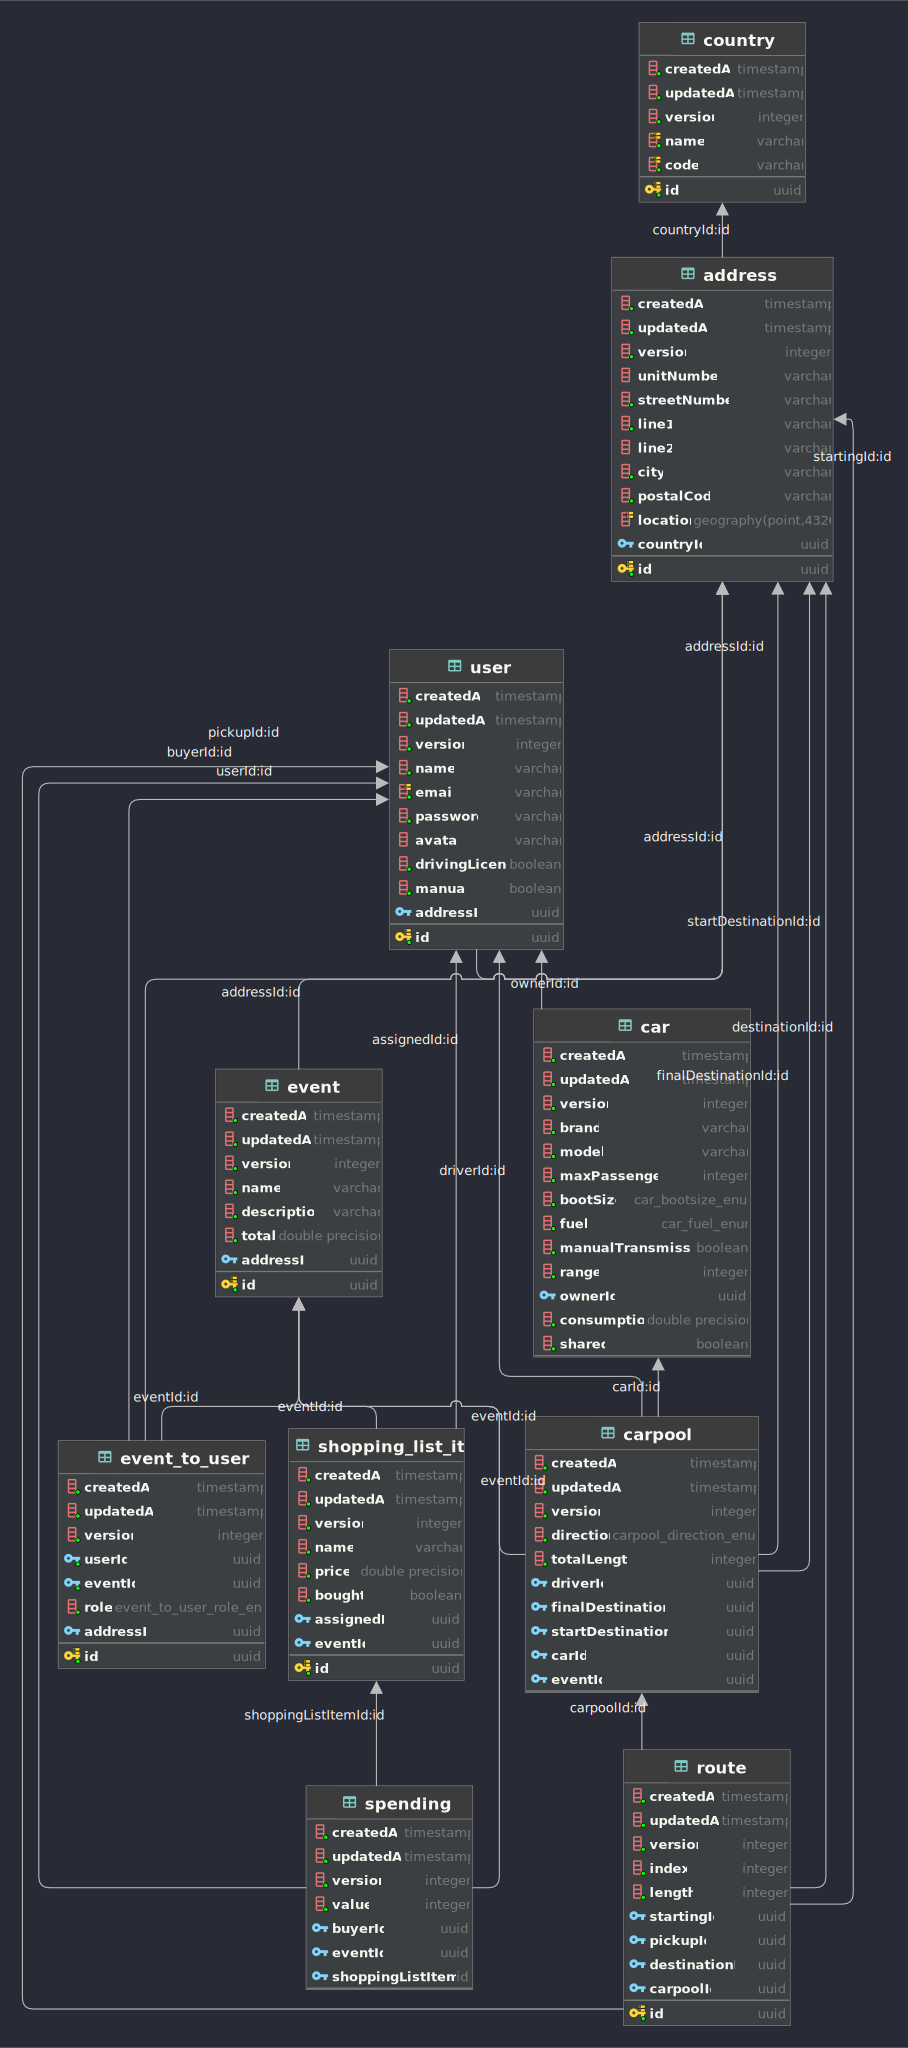
\includegraphics[width=\linewidth]{./images/dbShema}\caption{Architecture de la base de donnée}\label{fig:dbSchema2}
    \centering
\end{figure}

    \newpage


    \section{Historique du projet}\label{sec:historique-du-projet}
    \subsection{Introduction}\label{subsec:introduction2}
Dans cette section, nous examinerons l'évolution du projet, depuis sa phase de conceptualisation jusqu'à sa réalisation finale, en soulignant les différentes difficultés rencontrées en cours de route.
Nous mettrons également en lumière les jalons clés du projet, les ajustements de la planification et les interactions avec le rapporteur.

\subsection{Chronologie du projet}\label{subsec:chronologie-du-projet}
Le projet a officiellement débuté en septembre 2022, marqué par une première phase d'échanges intenses avec de potentiels utilisateurs et de définition des objectifs.
Des étapes clés ont jalonné notre progression, telles que la finalisation du cahier des charges et la sélection des technologies en octobre 2022,
le commencement du développement dans la même période, et enfin, le déploiement de la premiere version l'application en juin 2023.

\subsection{Réunions et interactions avec le client/rapporteur}\label{subsec:reunions-et-interactions-avec-le-client/rapporteur}
Au cours du projet, j'ai eu plusieurs réunions avec mon rapporteur.
Ces réunions ont été l'occasion de discuter de l'avancement du projet, de recueillir des retours constructifs et d'adapter notre approche en conséquence.
Par exemple, lors de la réunion de validation du sujet en octobre, nous avons convenu que la conception de l'application
devrait être suffisamment flexible pour permettre l'ajout de nouvelles fonctionnalités à l'avenir, comme un système de covoiturage.

\subsection{Évolution des choix techniques et stratégiques}\label{subsec:evolution-des-choix-techniques-et-strategiques}
Au fil du projet, certaines modifications ont été nécessaires.
Ces ajustements étaient principalement dus à RxJS. Initialement, j'avais prévu de concevoir le projet de manière à ce que l'application soit réactive sur l'ensemble du stack.
Cependant, après une discussion éclairante avec mon rapporteur, M. Noel,
nous avons décidé de construire le projet de manière classique tout en envisageant l'ajout de la réactivité dans une phase future.
    \newpage


    \section{Gestion de version et Intégration et Déploiement Continu}\label{sec:gestion-de-version-et-integration/-deploiement-continu}
    \subsection{Gestion de version}\label{subsec:gestion-de-version}

La gestion de version, ou versioning, est une pratique essentielle dans tout projet de développement.
Pour ce projet, nous avons utilisé Git comme système de gestion de versions et GitHub pour héberger notre code source.

Au départ du projet, j'ai choisi d'utiliser une seule branche pendant la majeure partie de la première phase.
Cette approche était suffisante pour répondre aux besoins du projet à ce stade, permettant de maintenir une simplicité de gestion.

Cependant, une fois le projet publié sur DockerHub et la mise en place du CI/CD, il est devenu évident que l'utilisation d'une seule branche n'était plus la meilleure option.
J'ai alors créé une branche de développement distincte.
Cette branche a permis de tester et de sauvegarder le code sans perturber la version en production.

Pour la rédaction de ce rapport, j'ai également créé une branche spécifique.
Cette approche a permis de travailler sur le rapport sans interférer avec le code de l'application.

Pour la gestion de l'infrastructure du projet, un second repository GitHub a été utilisé.
Ce choix a été motivé par le fait que l'infrastructure du projet était basée sur un autre projet existant que j'ai forké.
Ce repo distinct pour l'infrastructure a permis de maintenir une séparation claire entre le code de l'application et la gestion de l'infrastructure.

\subsection{Intégration et déploiement continu (CI/CD)}\label{subsec:integration-et-deploiement-continu-(ci/cd)}

Pour l'intégration continue (CI), j'ai mis en place des tests automatisés sur une grande partie des composants du backend et du frontend.

\begin{figure}[H]
    \begin{minipage}[b]{0.5\textwidth}
        \centering
        \includegraphics[height=0.3\textheight, keepaspectratio]{images/ci_workflow}
        \caption{Workflow d'intégration continue}
        \label{fig:ci_workflow}
    \end{minipage}%
    \begin{minipage}[b]{0.5\textwidth}
        Le workflow de CI est le suivant :

        \begin{itemize}
            \item Lint du code : vérification des erreurs de syntaxe.
            \item Build du code : si aucune erreur de linting n'est détectée, je peux construire le code.
            \item Tests unitaires et d'intégration : si le code se construit correctement, je lance les tests.
            \item Construction de l'image Docker : si les tests passent, je construis l'image du conteneur.
            \item Publication de l'image : si la construction de l'image réussit, je la publie sur DockerHub (seulement si je suis sur la branche principale).
        \end{itemize}
    \end{minipage}
\end{figure}

Pour le déploiement continu (CD), j'utilise un conteneur Watchtower qui, via le socket Docker,
vérifie régulièrement quelle version du conteneur est utilisée et si elle correspond bien à celle demandée.
Watchtower vérifie également la signature du conteneur en plus de son tag,
ce qui lui permet de mettre à jour un conteneur avec le tag "latest" lorsque l'image change.
Watchtower compare régulièrement la version courante des conteneurs contre celle hébergée sur DockerHub et si elles ne correspondent pas,
alors le conteneur est mis à jour.

\subsection{Conclusion}\label{subsec:conclusion}

La gestion de version a été un aspect crucial de ce projet.
L'adoption d'une approche adaptative, passant d'une seule branche à plusieurs branches en fonction des besoins du projet, a prouvé son efficacité.
De même, l'implémentation des pratiques de CI/CD a grandement amélioré le flux de travail et la qualité de
l'application, rendant le processus de développement plus fluide et fiable.
    \newpage


    \section{Produit Fini et Démonstration}\label{sec:produit-fini-et-demonstration}
    \subsection{État Actuel du Produit}\label{subsec:etat-actuel-du-produit}

Le produit actuel est une version minimale viable (MVP) de l'application web "Clever Party Thrower".
Il s'agit d'une application en cours de développement, mais qui dispose déjà de plusieurs fonctionnalités clés, dont l'envoi d'invitations,
la gestion des participants, le mécanisme de dettes, le vote pour les dates et la liste de courses.\\

Le système de covoiturage est presque achevé, mais manque encore de l'interface et du système de calcul de distance.
Des fonctionnalités telles que la double authentification et le mécanisme d'email sont par contre disponibles et opérationnelles.

\subsection{Installation du Produit}\label{subsec:installation-du-produit}

Une procédure d'installation détaillée est fournie dans le fichier README sur le dépôt GitHub.
Cependant, pour une compréhension rapide,
voici une vue d'ensemble des étapes nécessaires pour installer le produit :

\begin{enumerate}
    \item Prérequis : Docker doit être installé sur la machine.
    \item Étapes d'installation :
    \begin{enumerate}
        \item Téléchargez le fichier docker-compose disponible sur le dépôt GitHub et placez-le sur la machine hôte de l'application.
        \item Modifiez les variables d'environnement comme indiqué dans le fichier ou créez un nouveau fichier d'environnement avec les valeurs appropriées.
        \item Lancez la commande : \texttt{docker-compose up -d}.
    \end{enumerate}
\end{enumerate}

Pour plus de détails ou pour résoudre les problèmes d'installation, veuillez consulter le fichier README sur le dépôt GitHub.

\subsection{Démonstration du Produit}\label{subsec:demonstration-du-produit}

Une démonstration du produit a été préparée pour montrer son fonctionnement.
Cette démonstration met en évidence les fonctionnalités existantes de l'application, y compris la création d'un nouvel événement et la gestion des invitations.\\

Les retours positifs reçus jusqu'à présent indiquent que l'application répond déjà à
un besoin réel et qu'elle a le potentiel de devenir un outil précieux pour l'organisation de fêtes.

\subsection{Challenges et Améliorations Futures}\label{subsec:challenges-et-ameliorations-futures}

Il y a eu plusieurs défis lors du développement de ce projet.
L'un des plus notables a été l'incapacité à héberger l'application sur un cluster Kubernetes géré via Ansible,
malgré de nombreux efforts pour résoudre ce problème.
C'est une amélioration importante à réaliser à l'avenir, car elle permettra une haute disponibilité de l'application.\\

D'autres améliorations seraient : la finalisation du système de covoiturage, l'introduction de fonctionnalité supplémentaire comme l'intégration d'un chat
et l'amélioration de l'interface utilisateur.

\subsection{Points de Fierté}\label{subsec:points-de-fierte}

Je suis particulièrement fier de la qualité du code sur le back-end et sur le front-end.
J'ai investi beaucoup de temps et d'efforts pour m'assurer que le code soit propre, bien documenté et conforme aux bonnes pratiques de programmation.
Je suis convaincu que ces efforts paieront sur le long terme, en facilitant la maintenance et l'évolutivité de l'application.
    \newpage


    \section{Bilan}\label{sec:bilan}
    \subsubsection{Analyse critique du projet}\label{subsubsec:analyse-critique}

Le développement de ce projet a mis en lumière divers points forts et quelques zones à améliorer.

\textbf{Points forts:}
\begin{itemize}
    \item \textbf{Qualité du code :} Un investissement conséquent en temps a été consacré à produire un code de qualité, bien structuré, documenté et conforme aux meilleures pratiques de programmation.
    \item \textbf{CI/CD :} L'intégration et le déploiement continus ont démontré leur valeur en contribuant au maintien de la qualité du code et en accélérant le processus de développement.
    \item \textbf{TypeOrm :} L'utilisation de TypeOrm a facilité les itérations rapides sur la structure des données.
    \item \textbf{NestJs :} Le choix d'utiliser NestJs a permis d'ajouter rapidement des fonctionnalités au back-end.
    \item \textbf{Angular :} L'utilisation d'Angular a facilité la construction rapide d'une interface tout en simplifiant les tests.
\end{itemize}

\textbf{Points faibles:}
\begin{itemize}
    \item \textbf{Infrastructure :} L'implémentation de l'infrastructure, en particulier l'hébergement sur un cluster Kubernetes géré via Ansible, a représenté un défi majeur.
    \item \textbf{Fonctionnalités non terminées :} Certaines fonctionnalités, telles que le système de covoiturage et le mécanisme d'email, ne sont pas encore opérationnelles.
    \item \textbf{Interface utilisateur :} Certains composants de l'interface utilisateur pourraient être améliorés grâce à des animations.
\end{itemize}

\subsubsection{Améliorations envisageables}\label{subsubsec:ameliorations}

Le projet pourrait être amélioré à l'avenir dans plusieurs domaines.

\begin{itemize}
    \item \textbf{Infrastructure :} Résoudre le problème d'hébergement sur le cluster Kubernetes géré via Ansible serait bénéfique.
    \item \textbf{Fonctionnalités :} Il serait avantageux de finaliser le système de covoiturage et de mettre en place la double authentification ainsi que le mécanisme de validation d'email.
    \item \textbf{Interface utilisateur :} L'interface utilisateur pourrait être améliorée pour une meilleure convivialité, peut-être en adoptant un framework d'interface utilisateur plus moderne.
\end{itemize}

\subsubsection{Plan pour le futur}\label{subsubsec:plan-futur}

Dans le futur, je prévois de continuer à développer et améliorer ce projet.
Mon intention est de résoudre les problèmes d'infrastructure existants, de terminer les fonctionnalités inachevées et d'améliorer l'interface utilisateur.
J'envisage également d'ajouter des fonctionnalités telles qu'une playlist Spotify partagée pour l'événement, un chat instantané, et un mécanisme de partage d'images.

\subsubsection{Ce que j'aurais fait autrement}\label{subsubsec:ce-que-j-aurais-fait-autrement}

Avec le recul, j'aurais abordé certains aspects du projet différemment.
J'aurais, par exemple, commencé à travailler sur l'infrastructure plus tôt dans le processus de développement pour éviter certains des problèmes rencontrés.
De plus, je remets en question le choix de TypeScript pour le développement de l'application.
Ayant eu l'occasion d'apprendre Go et de découvrir les principes de Rust, je suis convaincu que l'utilisation de l'un de ces langages aurait pu faciliter le développement, notamment en ce qui concerne la gestion des erreurs.
De plus, bien que NestJs présente de nombreux points forts, il souffre des limitations de l'environnement JavaScript et du manque de typage fort sur plusieurs aspects.
Si je n'avais pas utilisé Go ou Rust, mon deuxième choix aurait été Kotlin avec Spring.
Comme mentionné dans mon analyse, cette combinaison offre de nombreux avantages.


En conclusion, je réalise que le développement d'une application nécessite une planification détaillée et une exécution rigoureuse.
Sur un plan plus personnel, je constate qu'il est bénéfique pour moi de me fixer de petits objectifs à court terme pour optimiser ma productivité.
À l'avenir, je m'efforcerai d'appliquer les leçons apprises de ce projet pour améliorer mes futurs efforts de développement.


    \section{Ressources utilisee}\label{sec:ressources-utilisee}
    Les ressources suivantes ont été déterminantes dans le développement de ce projet :

\subsection{Outils de développement}\label{subsec:outils-de-developpement}
\begin{itemize}
    \item \textbf{Docker :} A facilité la conteneurisation de l'application, optimisant ainsi la gestion et le déploiement~\cite{DockerDoc:online}.
    \item \textbf{Ansible :} A permis l'automatisation de la gestion des configurations, rendant le déploiement de l'infrastructure plus aisé~\cite{AnsibleDoc:online}.
    \item \textbf{GitHub :} A servi pour le contrôle de version, la gestion de projets et comme dépôt de code.
    \item \textbf{Github workflows :} A garanti un cycle de développement plus fluide grâce à l'intégration et le déploiement continus.
\end{itemize}

\subsection{Langages de programmation}\label{subsec:langages-de-programmation}
\begin{itemize}
    \item \textbf{TypeScript :} Langage principal pour le développement de l'application.
    \item \textbf{HTML/CSS/SCSS :} Impliqués dans la conception de l'interface utilisateur.
    \item \textbf{YAML/Jinja :} Employés pour la configuration de Kubernetes et dans le playbook Ansible.
    \item \textbf{Markdown :} Utilisé pour la création des différents fichiers Readme.
    \item \textbf{LaTex :} Utilisé pour la rédaction de ce rapport.
\end{itemize}

\subsection{Frameworks et bibliothèques JavaScript}\label{subsec:frameworks}
\begin{itemize}
    \item \textbf{NestJs :} Facilité le développement du back-end de l'application.
    \item \textbf{Angular :} Employé pour construire l'interface utilisateur et mettre en œuvre les tests.
    \item \textbf{TypeOrm :} Simplifié la gestion de la base de données.
    \item \textbf{PassportJs :} Utilisé pour la gestion de l'authentification.
    \item \textbf{Material UI :} Utilisé pour créer les composants de l'interface sur le front-end.
    \item \textbf{Apollo Angular :} Permis la communication avec l'API GraphQL du back-end.
    \item \textbf{Apollo Server :} A facilité la création de l'API GraphQL et la gestion des requêtes sur le back-end.
\end{itemize}

\subsection{APIs tierces}\label{subsec:apis-tierces}
\begin{itemize}
    \item \textbf{Open Street Map :} Cette API sera utilisée pour calculer les distances pour les covoiturages.
    \item \textbf{Spotify :} Potentiellement utilisée dans le futur.
    \item \textbf{Dicebear :} Utilisée pour générer des avatars pour les utilisateurs.
    \item \textbf{RestCountries :} Utilisée pour remplir la base de donnees avec tout les pays disponible.
\end{itemize}

\subsection{Autres ressources}\label{subsec:autres-ressources}
\begin{itemize}
    \item \textbf{Stack Overflow et Stack Exchange :} Sources précieuses de connaissances pour résoudre des problèmes spécifiques.
    \item \textbf{Documentations officielles :} Les documentations officielles d'Angular, NestJs, TypeOrm, Material UI, Apollo Angular, et K3S ont été des guides essentiels.
    \item \textbf{Chaîne YouTube de TechnoTim :} Principale source d'inspiration pour le cluster Kubernetes.
    Disponible sur : \url{https://www.youtube.com/@technotim}
    \item \textbf{Dépôt Git de TechnoTim :} Ce dépôt a servi de base pour la création du cluster Kubernetes.
    Disponible sur : \url{https://github.com/techno-tim/k3s-ansible}
\end{itemize}

Ces ressources ont joué un rôle crucial dans la réalisation de ce projet, contribuant à chaque étape du processus de développement.s de développement.


    \section{Conclusion}\label{sec:conclusion}

    Ce projet a été un voyage d'apprentissage et de découverte,
    fournissant des opportunités précieuses pour explorer les différentes technologies et pratiques de développement.
    Le développement de "Clever Party Thrower" a permis de mieux comprendre comment créer une application web complète,
    de la structuration du code à l'architecture de l'infrastructure.

    Malgré certains défis rencontrés, notamment dans l'implémentation de l'infrastructure et la finalisation de certaines fonctionnalités,
    le projet est bien avancé.
    Le code est bien structuré et documenté, et certaines des fonctionnalités clés sont déjà opérationnelles.

    Les prochaines étapes pour ce projet incluent la résolution des problèmes d'infrastructure,
    la finalisation des fonctionnalités inachevées, et l'amélioration de l'interface utilisateur.
    De nouvelles fonctionnalités, telles qu'une playlist Spotify partagée, un chat instantané,
    et un mécanisme de partage d'images, sont également envisagées.

    En rétrospective, il y a des aspects du projet qui auraient pu être abordés différemment,
    mais chaque défi et chaque erreur ont fourni une occasion d'apprendre et de grandir en tant que développeur.
    Ces leçons seront inestimables pour les futurs projets de développement.

    En somme, "Clever Party Thrower" est une application prometteuse avec un potentiel considérable.
    Alors que le projet continue d'évoluer et de s'améliorer, il est excitant de penser à toutes les possibilités futures qu'il offre.


    %\backendx
    % La db (shema+ ORM + GDPR)
    % graphql
    % NestJs

    % Le front end
    % agular
    % apollo
    % les service
    % l'authentification par token


%    \section{hebergement}
    % proxmox
    % ansible
    % kubernetes
    % traefik, certmanager & https
    % longhorn & rancher
    % reseau (ce qui aurais du etre fait et ce qui est fait)
%   docekr-compose
\end{document}
